\documentclass{beamer}

\usepackage{txfonts}
\usepackage{hyperref}
\usepackage{fancybox}
\usepackage{xfrac}
\usepackage{cancel}


\newcommand{\heart}{\ensuremath\heartsuit}

\usepackage{mathtools,amssymb}
\newcommand{\myarrow}{\scalebox{2}[2]{$\mathclap{\curvearrowleft}\mkern2.2mu
                                                 \mathclap{\curvearrowright}$}}

\DeclareMathOperator{\Bin}{\mathrm{Bin}}

\hypersetup{colorlinks=false,linkbordercolor=red,linkcolor=green,pdfborderstyle={/S/U/W 1}}

\addtobeamertemplate{navigation symbols}{}{ \hspace{1em}    \usebeamerfont{footline}%
    \insertframenumber / \inserttotalframenumber}

\geometry{papersize={15cm,13cm}}
\usepackage{lipsum}

\makeatletter
\newenvironment<>{contdproof}[1][\proofname]{%
    \par
    \def\insertproofname{#1\@addpunct{.}}%
    \usebeamertemplate{proof begin}#2}
  {\usebeamertemplate{proof end}}
\makeatother


\setbeamertemplate{theorems}[numbered]

\newtheorem*{nonumdefinition}{Definition}
\newtheorem*{nonumproblem}{Problem}
\newtheorem*{nonumlemma}{Lemma}
\newtheorem*{nonumtheorem}{Theorem}
\newtheorem*{nonumproof}{Proof}
\newtheorem*{nonumremark}{Remark}
\newtheorem*{answer}{Answer}
\newtheorem*{nonumremarks}{Remarks}
\newtheorem*{nonumexamples}{Examples}
\newtheorem*{nonumsolution}{Solution}
\newtheorem*{nonumexample}{Example}
\newtheorem*{nonumproposition}{Proposition}

\newtheorem{remark}{Remark}
\newtheorem{exam}{Example}




\theoremstyle{alphtheorem}
\newtheorem{alphtheorem}{Theorem}
\renewcommand{\thealphtheorem}{\Alph{alphtheorem}}
\renewcommand{\thesection}{\arabic{section}}



\usepackage{tikz}
\newcommand*\mycirc[1]{%
  \tikz[baseline=(C.base)]\node[draw,circle,inner sep=.7pt](C) {#1};\:
}

\newcommand\myheading[1]{%
  \par\bigskip
  {\color{blue}{\large #1}}\par\smallskip}

%\usetheme{Warsaw}
%\usetheme{Berkeley} %sample 1

\usetheme{Berlin} % sample 2
%\usetheme{AnnArbor} % sample 3

\let\otp\titlepage
\renewcommand{\titlepage}{\otp\addtocounter{framenumber}{-1}}

\title{Lecture 20: Stat 400, Lecture 20 Random Sainples (\S 5.3)}
\author{}
\date{}

\begin{document}
\begin{frame}[plain]
\titlepage
\end{frame}

\begin{frame}
One of the most important concepts in statistics is that of a ``random sample''. The definition of a random sample is rather abstract. However it is critical to understand the idea behind the definition, so we will spend an entire lecture motivating the definition we will do this by giving three motivating examples: polling for elections, testing the lifetime of a Gateway computer, and picking a sequence of random numbers.
\end{frame}

\begin{frame}
\myheading{First Motivating Example}

We recall that a random variable $X$ is a Bernoulli random variable if $X$ takes exactly two values 0 and 1 such that 
\begin{align*}
& P(X=1) = p \\
& P(X=0) = q \qquad q =1-p
\end{align*}
In this case we write $X \sim b (1,p)$ (the Bernoulli distribution is a special case of the binomial distribution).

We define a Bernoulli random variable $X_{\text{election}}$ as follows.

Choose a random voter in the U.S. ASK him (her) if he (she) intends to vote for Gore in the next election Record 1 if yes and 0 if no. So $X_{\text{election}}$ takes.
\end{frame}

\begin{frame}
valves 1 an 0 with some ??? (but unknown to us) probabilities $p$ and $q$.

\myheading{The \$ 64,000 question}

What is $p$?

How do you answer this question? Take a poll - in the language of statistics we say one is ``taking a sample from a $b(1,p)$ distribution where $p$ is unknown.''

If we poll $n$ people we arrive at a sequence of 0's and 1's
$$
X_1, X_2,  \ldots, X_n
$$
We can represent this schematically by 

\medskip
\centerline{\includegraphics{figure/art20(1).eps}}
\end{frame}

\begin{frame}
We think of $X_1, X_2, \ldots, X_n$ as the results {\it after the poll is taken} we now introduce {\it random variables} $X_1, X_2, \ldots, X_n$ representing the potential outcomes {\it before the poll is taken} - we assume we have decided how many people we will talk to.

Thus taking a poll assigns definite values $X_1, X_2, \ldots, X_n$ to the random variables $X_1, X_2, \ldots, X_n$. We may schematically represent the situation before the poll is taken by 

\medskip
\centerline{\includegraphics{figure/art20(2).eps}}

The dotted arrow means we have not yet performed the poll.
\end{frame}

\begin{frame}
It is critical to observe that $X_1, X_2, \ldots, X_n$ are {\it random} variables ($X_1, X_2, \ldots, X_n$ are ordinary variables). They take values 0 and 1 with probabilities $q$ and $p$ respectively. So the $X_1'$s have the same probability distribution as the ``underlying'' (i.e. the case we are sampling from) random variable $X_{\text{election}}$ (if the poll is constructed properly).
Note also the random variables $X_1, X_2, \ldots, X_n$ are independent and ``identically distributed.'' We say $X_1, X_2, \ldots, X_n$ is a random sample from a $\Bin(1,p)$ distribution.
\end{frame}

\begin{frame}
We conclude this example with a formal mathematical definition of $X_1, X_2, \ldots, X_n$. The sample space $S$ of the above poll (``experiment'') is the set of all $n$-tuples ($X_1, X_2, \ldots, X_n$) of 0's and 1's. It is the same as the sample space for $n$ flips of a weighted coin. There is a probability function $P$ defined on $S$. For example, 
$$
P(0,0,0) = q^n
$$
The random variables $X_1, X_2, \ldots, X_n$ are defined to be functions on $S$ defined by 
$$
X_i (x_1, \ldots, x_n) = X_i
$$
So they are random variables - a random variable is a function on a probability space.
\end{frame}

\begin{frame}
\myheading{Second Motivating Example}

Suppose now we wish to study the expected life of a Gateway computer so in this case we would be studying the random variable $X_{\text{Gateway}}$ which is defined as follows.

\medskip
($X_{\text{Gateway}} =t$) means that a randomly selected Gateway computer fails at time $t$. A good model for the distribution of $X_{\text{Gateway}}$ is an exponential distribution with a definite but unknown mean $\mu = \dfrac{1}{\lambda}$.

\myheading{The new \$ 64,000 Question}

What is $\mu$?

How do you answer this question? You get hold of a number of 
\end{frame}

\begin{frame}
Gateway computers and run them until they break down. You record these results. We may represent the results schematically by 

\medskip
\centerline{\includegraphics{figure/art20(3).eps}}

Once again, we introduce variables $X_1, X_2, \ldots, X_n$ (after we have decided how many computers we are going to look at) before we actually look at computers. So schematically we have the ``before picture''.

\medskip
\centerline{\includegraphics{figure/art20(4).eps}}

After we test $n$ computers we assign definite values to $X_1, X_2, \ldots, X_n$.
\end{frame}

\begin{frame}
Again, $X_1, X_2, \ldots, X_n$ are random variables with the same probability distribution as the underlying random variable $X_{\text{Gateway}}$.

\medskip
Assuming that our test is correctly designed, $X_1, X_2, \ldots, X_n$ will be independent we say $X_1, X_2, \ldots, X_n$ is a random sample from an exponential distribution with parameter.

\medskip
Once again we have a formal mathematical definition. The sample space $S$ of the experiment is now the set of all $n$-tuples $(X_1, X_2, \ldots, X_n)$ of positive real numbers, the possible break-down times for the $n$-computer, to be tested. $S$ is a probability space (but not discrete). We define 
\end{frame}

\begin{frame}
The random variables $X_1, X_2, \ldots, X_n$ is as functions on $S$ as before:
$$
X_i (x_1, \ldots, x_n) = x_i
$$

\myheading{Third Motivating Example}

Our third motivating example will be the experiment of ``choosing $n$ random numbers from the interval $[0,1]$''. We have seen that a good model for ``choosing a random number from $[0,1]$'' is the uniform distribution $\cup (0,1)$, precisely we let

$X=a$ random number in $[0,1]$. Then $P(a \leq X \leq b) = b-a$ (assuming $0 \leq a \leq b \leq 1$)
\end{frame}

\begin{frame}

\medskip
\centerline{\includegraphics{figure/art20(5).eps}}

We can repeat the experiment $n$ times. After we actually perform the experiment $n$ times, we obtain $n$ definite numbers $X_1, X_2, \ldots, X_n$ in $[0,1]$.

\medskip
\centerline{\includegraphics{figure/art20(6).eps}}

 
\textbf{\textit{Before}} we make the choices we have variables $X_1, X_2, \ldots, X_n$ representing the first, second, $\ldots$, $n$-th choice. Schematically we have

\medskip
\centerline{\includegraphics{figure/art20(7).eps}}
\end{frame}

\begin{frame}
We note that $X_1, X_2, \ldots, X_n$ all have $\cup (0,1)$-distribution and are all independent we say $X_1, X_2, \ldots, X_n$ is a random sample from $\cup (0,1)$.

Once again we have the formal mathematical definition
$$
S = \{(X_1, X_2, \ldots, X_n): X_i \in [0,1]\}
$$
$X_i : S \to [0,1]$ where  $X_i (X_1, X_2, \ldots, X_n) = X_i =$ ``$i$-th choice'' so $X_i$ is a $\cup (0,1)$-random variable Hopefully we have motivated:

\myheading{Definition (pg. 20)}
A random sample of size $n$ is a sequence $X_1, X_2, \ldots, X_n$ of random variables such that 
\end{frame}

\begin{frame}
\begin{itemize}
\item[(i)] $X_1, X_2, \ldots, X_n$ are independent 

AND

\item[(ii)] $X_1, X_2, \ldots, X_n$ all have the same probability distribution.
\end{itemize}

The common probability distribution will be called the ``underlying distribution''-it is the one we are sampling from.

\textit{Def.}

A statistic is a random variable that is a function (i.e. combination) of $X_1, X_2, \ldots, X_n$.

The following statistics will be very important to us.
\begin{itemize}
\item[(1)] The sample total $T_0$ defined by 
$$
T_0 = X_1 + X_2 + \ldots + X_n
$$
\end{itemize}
\end{frame}

\begin{frame}
\begin{itemize}
\item[(2)] The sample mean 
$$
\overline{X} = \frac{1}{n} T_o = \frac{X_1 + X_2 + \ldots + X_n}{n}
$$

\item[(3)] The sample variance
$$
S^2 = \frac{1}{n-1} \left( \sum\limits^1_{i=1} (X_i - \overline{X})\right)^2
$$
\end{itemize}

\end{frame}
\end{document}




